\setcounter{section}{9}
\section{Глава 10. Кратные интегралы}
\subsection{Определение кратного интеграла}
\subsubsection{Случай, когда $f(x)$ - ограниченная функция.}
\begin{Def}
Пусть $f$ -- ограниченная функция, заданная на измеримом по Лебегу Жордану) множестве $E \subset \R^n$ конечной меры. 

$\textbf{Разбиением}$ множества $E$ называется $E=\bigsqcup\limits_{k=1}^N E_k$, где $E_k$ - измеримые по Лебегу (Жордану). \newline В качестве $\Delta x_k$ будем брать меру множеств $E_k$. 

Обозначим $M_k=\sup\limits_{x\in E_k} f\left(x\right) ,\  m_k=\inf\limits_{x\in E_k}f\left(x\right)$ \newline
Суммы Дарбу - Лебега (Жордана): верхняя $\mathcal{U}(P, f)=\sum\limits_{k=1}^N M_k \cdot \mu_{(J)}(E_k)$, нижняя $L(P, f)\?=\sum\limits_{k=1}^N m_k \cdot \mu_{(J)}(E_k)$.
\newline Верхний интеграл Лебега или Римана (L)(R)$\ \overline{I}_E(f)=\inf\limits_P \mathcal{U}(P, f)$,\newline Нижний интеграл Лебега или Римана (L)(R)$\ \underline{I}_E(f)=\sup\limits_P L(P, f)$
\end{Def}
\begin{Def}
Если (R)$\ \overline{I}_E(f)=$ (R)$\ \underline{I}_E(f)$, то $f$ называется интегрируемой по Риману на $E$, $\int\limits_E f(x)dx=$ (R)$\ \overline{I}_E(f)$ \newline
Если (L)$\ \overline{I}_E(f)=$ (L)$\ \underline{I}_E(f)$, то $f$ называется интегрируемой по Лебегу на $E$, $\int\limits_E f(x)d\mu (x)\?= \text{(L) }\overline{I}_E(f)$
\end{Def}
\textbf{Утв. 1} Функция $f$ интегрируема по Риману на $[a,b]$(в смысле старого определения) $\Leftrightarrow$ $f$ интегрируема по Риману на $E=[a,b] \subset \R^1$.
\begin{proof}
$(\Rightarrow)$	Составим цепочку неравенств:
\begin{equation}
\underline{I}(f) \overset{(1)}{\leqslant} \text{(R) }\underline{I}_{[a,b]}(f)\overset{(2)}{\leqslant} \text{(L) }\underline{I}_{[a,b]}(f)\overset{(3)}{\leqslant}\text{(L) } \overline{I}_{[a,b]}(f) \overset{(4)}{\leqslant} \text{(R) } \overline{I}_{[a,b]}(f)\overset{(5)}{\leqslant} \overline{I}(f)\tag{10.1.1}\label{10.1.1} 
\end{equation}

Неравенство (1) следует из того, что в старом определении мы делили на отрезки, которые пересекаются в концах, а в новом определении идет разбиение на непересекающиеся, измеримые по Жордану множества.

Неравенство (2) следует из того, что нижние интегралы в смысле Римана и в смысле Лебега отличаются тем, на какие множества мы разбиваем: измеримые по Жордану или Лебегу. Но так как каждое измеримое по Жордану автоматически измеримо по Лебегу, то в $\text{(L) }\underline{I}_{[a,b]}(f)$ мы берем точную верхнюю грань по большему множеству.

Неравенства (4), (5) следуют из выше доказанных, но в обратном порядке.

Доказательство неравенства (3): хотим установить, что для любых двух разбиений $P_1, P_2\ L(P_1, f) \leqslant \mathcal{U}(P_2, f)$, что и докажет требуемое неравенство. Для этого необходимо взять общее измельчение разбиений $P=P_1 \bigcup P_2$ и получить цепочку неравенств $L(P_1, f) \leqslant L(P, f) \leqslant \mathcal{U}(P, f) \leqslant \mathcal{U}(P_2, f)$. Получим это: составим два произвольных разбиения 
$P_1 : E = \bigsqcup\limits_{k=1}^{N_1} E_k^{(1)},\ P_2 : E = \bigsqcup\limits_{k=1}^{N_2} E_k^{(2)}$. Тогда общее измельчение $ P : E = \bigsqcup\limits_{k=1}^{N_1} \bigsqcup\limits_{j=1}^{N_2} E_k^{(1)} \bigcap E_j^{(2)}$.
Докажем неравенство для нижних сумм:

 $L(P_1, f)=\sum\limits_{k=1}^{N_1} \inf\limits_{x\in E_k^{(1)}}f(x) \cdot \mu_{(J)}(E_k^{(1)}) =
\sum\limits_{k=1}^{N_1} \inf\limits_{x\in E_k^{(1)}}f(x) \sum\limits_{j=1}^{N_2} \mu_{(J)} (E_k^{(1)}\bigcap E_j^{(2)})\?\leqslant \sum\limits_{k=1}^{N_1}\sum\limits_{j=1}^{N_2}\inf\limits_{x\in E_k^{(1)}\bigcap (E_j^{(2)}}f(x)\cdot \mu_{(J)} (E_k^{(1)}\bigcap E_j^{(2)})=L(P,f)$, так как инфимум по $E_k^{(1)}$ не превосходит инфимум по $E_k^{(1)}\bigcap E_j^{(2)}$ для каждого $j$. Аналогично доказывается оставшаяся часть неравенства.

Из доказанного неравенства \ref{10.1.1} следует, что из интегрируемости по Риману в старом смысле, мы получили интегрируемость в новом смысле, так как $\underline{I}(f) = \overline{I}(f)$, а также, что из интегрируемости по Риману следует интегрируемость по Лебегу.

$(\Leftarrow$)
Отступление.
Вспомним критерий интегрируемости:
$$f\in R[a,b] \Leftrightarrow (\forall \varepsilon > 0)(\exists P)\ \mathcal{U}(P, f)-L(P, f)<\varepsilon$$
В доказательстве мы использовали тот факт, что $\overline{I}(f)=\inf\limits_P \mathcal{U}(P, f)$, $\ \underline{I}(f)=\sup\limits_P L(P, f)$, и так как $\mathcal{U}(P, f)-L(P, f)<\varepsilon$, то и $\overline{I}(f) - \underline{I}(f) < \varepsilon$. Эта разность всегда неотрицательная, меньше любого положительного числа, значит равна 0. Вместо интегрируемости по Риману на отрезке можем написать интегрируемость по Риману на любом измеримом по Жордану или Лебегу.

Вернемся к доказательству.

 Пусть функция интегрируема по Риману в новом смысле: $\exists \int\limits_{[a,b]}f(x)dx$, тогда по критерию интегрируемости: $(\forall \varepsilon > 0)(\exists P:[a,b]=\bigsqcup\limits_{k=1}^{N} E_k) \mathcal{U}(P,f)-L(P,f)<\varepsilon$, где $E_k$ - измеримые по Жордану множества. Внутренняя мера Жордана $\mu_{*}^J(E_k)=\sup\limits_{M \subset E_k} |M|$, где $M$ - элементарное множество. Элементарным множеством на прямой является объединение конечного числа промежутков. Тогда 
$$\exists\text{ набор точек } \{a_j^{(k)}, b_j^{(k)}\},\ \bigsqcup\limits_{j=1}^{n_k}[a_j^{(k)}, b_j^{(k)}] \subset E_k,\ \mu_jE_k \backslash \bigsqcup \limits_{j=1}^{n_k}[a_j^{(k)}, b_j^{(k)}]) < \dfrac{\varepsilon}{2\cdot C \cdot N},$$
\mbox{где $|f(x)|\leqslant C$. Возьмем разбиение в старом смысле $Q: a=x_0 < x_1 < \ldots < x_{\nu} = b,$} $\text{где множество точек }\{x_i\}_{i=1}^{\nu} = \{a_j^{(k)}, b_j^{(k)}\}_{j=1}^{n_k},  k=\overline{1,\ldots,N}$.
Оценим $\mathcal{U}(Q, f)-L(Q, f)=\sum\limits_{i=1}^{\nu}(\sup\limits_{[x_{i-1}, x_i]}f(x)-\inf\limits_{[x_{i-1}, x_i]}f(x))\cdot \Delta x_i = \sum\limits_{k=1}^N \sum\limits_{j=1}^{n_k}(\sup\limits_{x\in [a_j^{(k)},b_j^{(k)}]}f(x)-\inf\limits_{x\in [a_j^{(k)},b_j^{(k)}]}f(x) )(b_j-a_j )+\sum\limits_{x\in B}(\sup\limits_{[x_{i-1}, x_i]}f(x)-\inf\limits_{[x_{i-1}, x_i]}f(x))\Delta x_i \leqslant \sum\limits_{k=1}^N(M_k-m_k)\sum\limits_{j=1}^{n_k}(b_j-a_j)+\sum\limits_{i\in B}\ldots \leqslant \sum\limits_{k=1}^N (M_k-m_k)\cdot \mu_{J}(E_k)+2\cdot C\cdot \sum\limits_{i\in B}\Delta x_i < 2\varepsilon$
\end{proof}
.
\begin{wrapfigure}{r}{0.5\linewidth}
	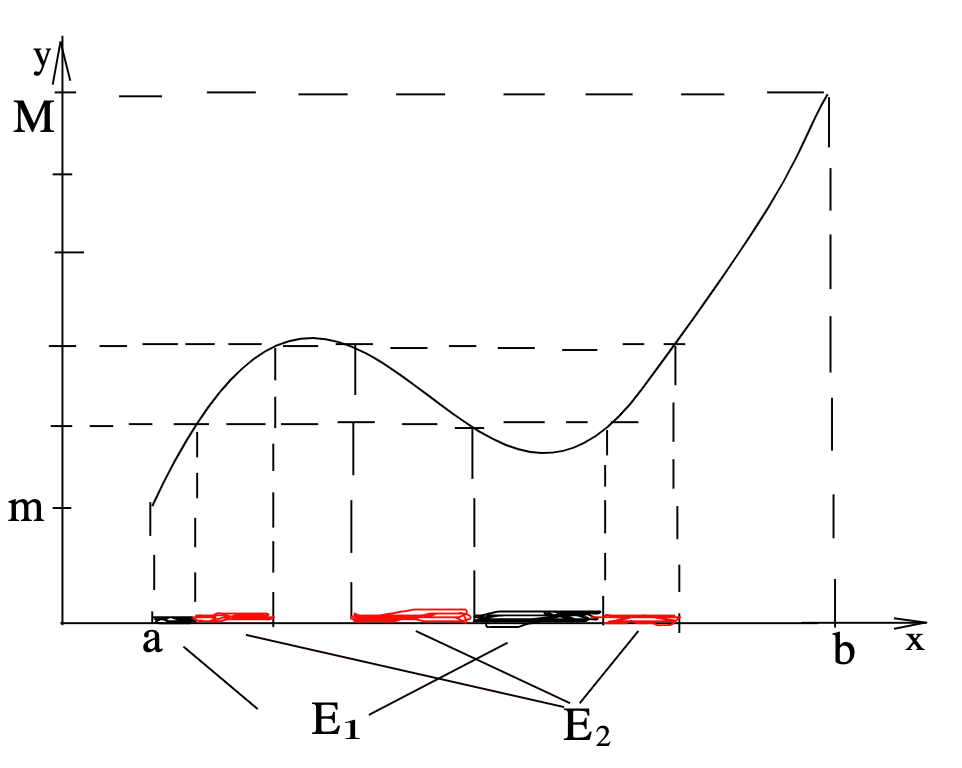
\includegraphics[width=\linewidth]{images/1.png}
\end{wrapfigure}
\begin{Def}
	\mbox{Пусть $ f:E\to\mathbb{R} $} ---  ограниченная измеримая на измеримом по Лебегу множестве \mbox{$ E\subset\mathbb{R}^n $} конечной меры функция.

	Если $ M=\sup\limits_{x\in E}f(x), $ $ m=\inf\limits_{x\in E}f(x), $ то \textbf{разбиением Лебега}, отвечающим разбиению $ Q=\{m=y_0<y_1<\ldots <y_N=M\}, $ называется разбиение
	$ P: E=\bigsqcup\limits_{i=1}^{N}E_i$, \mbox{где $E_i=\{x\in E: fx)\in [y_{i-1}, y_i)\},$} $i=1, \ldots, N-1$.
	\newline
	$E_N= \{x\in E: fx)\in [y_{N-1}, y_N]\}$
	\newline
	\newline
	\mbox{Тогда интегральной суммой Лебега назовем $S(Q, f, \{t_i\})=\sum\limits_{i=1}^N f(t_i)\mu(E_i)$, где $t_i \in E_i,$}$ 
	\newline i = 1, \ldots, N$.
\end{Def} 
\begin{theorem}(Основная теорема об интеграле Лебега от ограниченных функций).
	Если $f(x)$ ограниченная измеримая на измеримом по Лебегу множестве $ E\subset\R^n $ конечной меры  функция, то она интегрируема по Лебегу (суммируема) на $E$, причем ее интеграл равен пределу интегральных сумм с разбиениями Лебега, отвечающими разбиениям  $ Q $, при стремящемся к нулю диаметре последнего, т.е. $$\int\limits_E f(x)d\mu(x)=\lim_{\Delta(Q)\to 0}S(Q,f,\{t_i\}).$$
	Это значит, что $(\forall \varepsilon >0)(\exists \delta > 0)(\forall Q, \Delta(Q)<\delta) \text{ и } \forall \{t_i\}, t_i \in E_i, i=1,\ldots, N,$ где $E=\bigsqcup\limits_{i=1}^N E_i$ --- разбиение Лебега, отвечающее разбиению $Q$ отрезка $[m, M]$, выполняется $|S(Q, f, \{t_i\})-\int\limits_E f(x)d\mu(x)|<\varepsilon$.
\end{theorem}

\begin{proof}
	Прежде всего заметим, что если $P: E=\bigsqcup\limits_{i=1}^N E_i$, то\newline $L(P, f)\leqslant S(Q, f, \{t_i\})\leqslant \mathcal{U}(P, f)$. Кроме того $\mathcal{U}(P, f) - L(P, f) = \sum\limits_{i=1}^N(M_i-m_i)\mu(E_i) \?\leqslant \sum\limits_{i=1}^N (y_i-y_{i-1})\cdot\mu(E_i)\leqslant \Delta(Q) \sum\limits_{i=1}^N\mu(E_i)=\Delta(Q)\mu(E)$. В качестве $\delta = \dfrac{\varepsilon}{\mu(E)}$. Для множеств $ E $ меры нуль утверждение очевидно, так как все суммы (верхние, нижние, интегральные) в этом случае равны нулю.
\end{proof}

\subsubsection{Случай, когда $f(x)\geqslant 0$.}
Пусть $f(x)\geqslant 0$ - измеримая на измеримом по Лебегу множестве $E$ конечной меры функция. В качестве разбиений будем допускать и разбиения на счетное число измеримых по Лебегу множеств: $E = \bigsqcup\limits_{i=0 }^{\infty}E_i,\ E_0:=\{x\in E:f(x)=+\infty\}$. Обратите внимание! Индексацию ведем с 0, и $E_0$ жестко фиксируем. Соглашение: если $\mu(E_0)=0$, то $(+\infty)\cdot \mu(E_0)=0$. Получаем, что мы ничего не можем сказать о $M$, а $m=0$. 

Тогда разбиение принимает вид $Q: 0=y_0<y_1<\ldots$. 

В качестве $E_i = \{x\in E: f(x)\in[y_{i-1}, y_i)\}, i=1,\ldots$.

$\Delta(Q):=\sup\limits_{i=1, \ldots}(y_i-y_{i-1})$, может равняться и $+\infty$.

$L(P, f)=\sum\limits_{i=0}^{\infty}m_i\cdot \mu(E_i),\  \mathcal{U}(P, f)=\sum\limits_{i=0}^{\infty}M_i\cdot \mu(E_i)$ 

\begin{theorem}Основная теорема об интеграле Лебега для неограниченных измеримых функций)
Если $f(x)$ - неотрицательная, измеримая на измеримом по Лебегу множестве $E\subset \R^n$ конечной меры, то она интегрируема по Лебегу на $E$, причем
$\int\limits_E f(x)d\mu(x)\?=\lim\limits_{\Delta(Q)\to0}S(Q, f, \{t_i\}).$ 

При конечном значении интеграла понятие предела такого вида -- то же, что и в предыдущей основной теореме, если же интеграл бесконечен, то требуется, чтобы \newline$(\forall \varepsilon>0)( \exists \delta > 0)(\forall Q, \Delta(Q)<\delta) \text{ и } \forall \{t_i\}, t_i \in E_i, i=1,\ldots$, где $E=\bigsqcup\limits_{i=1}^{\infty} E_i$ --- разбиение Лебега, отвечающее разбиению $Q$ полуоси $[0, +\infty)$, выполняется $S(Q, f, \{t_i\})\geqslant\varepsilon$.
\end{theorem}

\begin{proof}
В случае конечного интеграла, доказательство аналогично доказательству предыдущей теоремы. Если интеграл бесконечен, то и предел интегральных сумм бесконечность, так как все $S$ зажаты между $\mathcal{U}(P, f) \:\text{и} \:L(P, f)$.
\end{proof}

\begin{Def}
Если $\int\limits_E f(x)d\mu(x) < +\infty$, то $f$ называется суммируемой на $E$.
\end{Def}

\subsubsection{Случай, когда $f(x)$ - любого знака.}
Пусть $f(x)$ измерима на измеримом по Лебегу множестве $E \subset \R^n$ конечной меры. Введем $f_+(x):=\max(f(x), 0), f_-(x):=\max(-f(x), 0)$ - это неотрицательные, измеримые функции. Такие функции интегрируемы по Лебегу, то есть существуют $\int\limits_E f_+(x)d\mu(x), \int\limits_E f_-(x)d\mu(x)$. Если хотя бы один из этих интегралов конечен, то $f$ называется интегрируемой по Лебегу. Если оба конечны, то $f$ - суммируемая на $E$.
$$\int\limits_E f_+(x)d\mu(x)- \int\limits_E f_-(x)d\mu(x) = \int\limits_E f(x)d\mu(x)$$
Пример измеримой, но не интегрируемой по Лебегу функции: возьмем отрезок, на одной его половине функция равна $+\infty$, на другой $-\infty$.


